\def \Subject {گام پنجم: درست کردن اسلاید ها}
\section{\Subject}
پس از جمع آوری اطلاعات و مقایسه با با پروتکل های دیگر حال به درست کردن اسلاید برای ارائه می پردازم.
\subsection{نرم افزار مورد استفاده}
در این بخش به نرم افزار به کار برده شده برای درست کردن اسلاید ها می پردازم. اسلاید ها باید به گونه ای باشند که بتوانند اطلاعات مورد نیاز را به خوبی منتقل کنند و در عین حال زیبا باشند. برای این کار از نرم افزار 
\lr{PowerPoint} 
استفاده می کنم. این نرم افزار از نظر زیبایی و سادگی کار بسیار مناسب است. اما از نظر امکانات و قابلیت های موجود در آن کمی ضعیف است. اما با این حال به نظر من از نظر کلی این نرم افزار برای این کار مناسب است. 
به همین علت تصمیم گرفتم که از این نرم افزار برای این کار استفاده کنم.
\subsection{مراحل درست کردن اسلاید}
\begin{itemize}
    \item {
        ابتدا مقدمه و معرفی مختصری راجع به موضوع ارائه می دهیم.
    }
    \item {
        سپس دلیل نامگذاری و علت بوجود آمدن را توضیح می دهیم.
    }
    \item {
        علاوه بر اطلاعات جمع آوری شده در مراحل قبل به جستجو برای یافتن عکس های مناسب می پردازیم.
        همچنین برای بعضی از تعاریف از منابعی کمک گرفتم که در آخر مستند قابل دیدن است.
    }
    \item {
        بعد به کاربرد های آن و انواع دستگاه های آن اشاره نمودم.
    }
    \item {
        سپس معماری شبکه آن و لایه های آن را با عکس هایی که پیدا کرده بودم توضیح دادم.
    }
    \item {
        ویژگی های امنیتی آن را بازگو کردم.
    }
    \item {
        در مرحله بعد به مقایسه آن با پروتکل های دیگر پرداختم.
    }
    \item {
        در آخرین مرحله هم منابع استفاده شده را ذکر کردم.
    }
\end{itemize}

\subsection{نمونه ای از اسلاید ها}
در زیر یکی از اسلاید های اولیه ارائه آورده شده است که در آن به معرفی مختصری از موضوع ارائه پرداخته شده است.
در این اسلاید میتوانید تم و رنگ های استفاده شده برای ساخت اسلاید ها را مشاهده کنید.
همان طور که مشاهده می کنید من از پس زمینه  سیاه به همراه رنگ های فیروزه ای و برای اسلاید ها استفاده کرده‌ام.
همچنین رنگ متن ها را هم به گونه ای انتخاب کرده ام که با پس زمینه سیاه سازگار باشد.
به همین دلیل از رنگ سفید برای متن ها استفاده کرده ام.
به علاوه از فونت هایی که در این اسلاید ها استفاده شده است می توان به فونت های
\lr{Arial}
،
\lr{Lato}
،
\lr{Century Gothic}
و
\lr{Nunito}
اشاره کرد.


\begin{figure}[H]
    \centering
    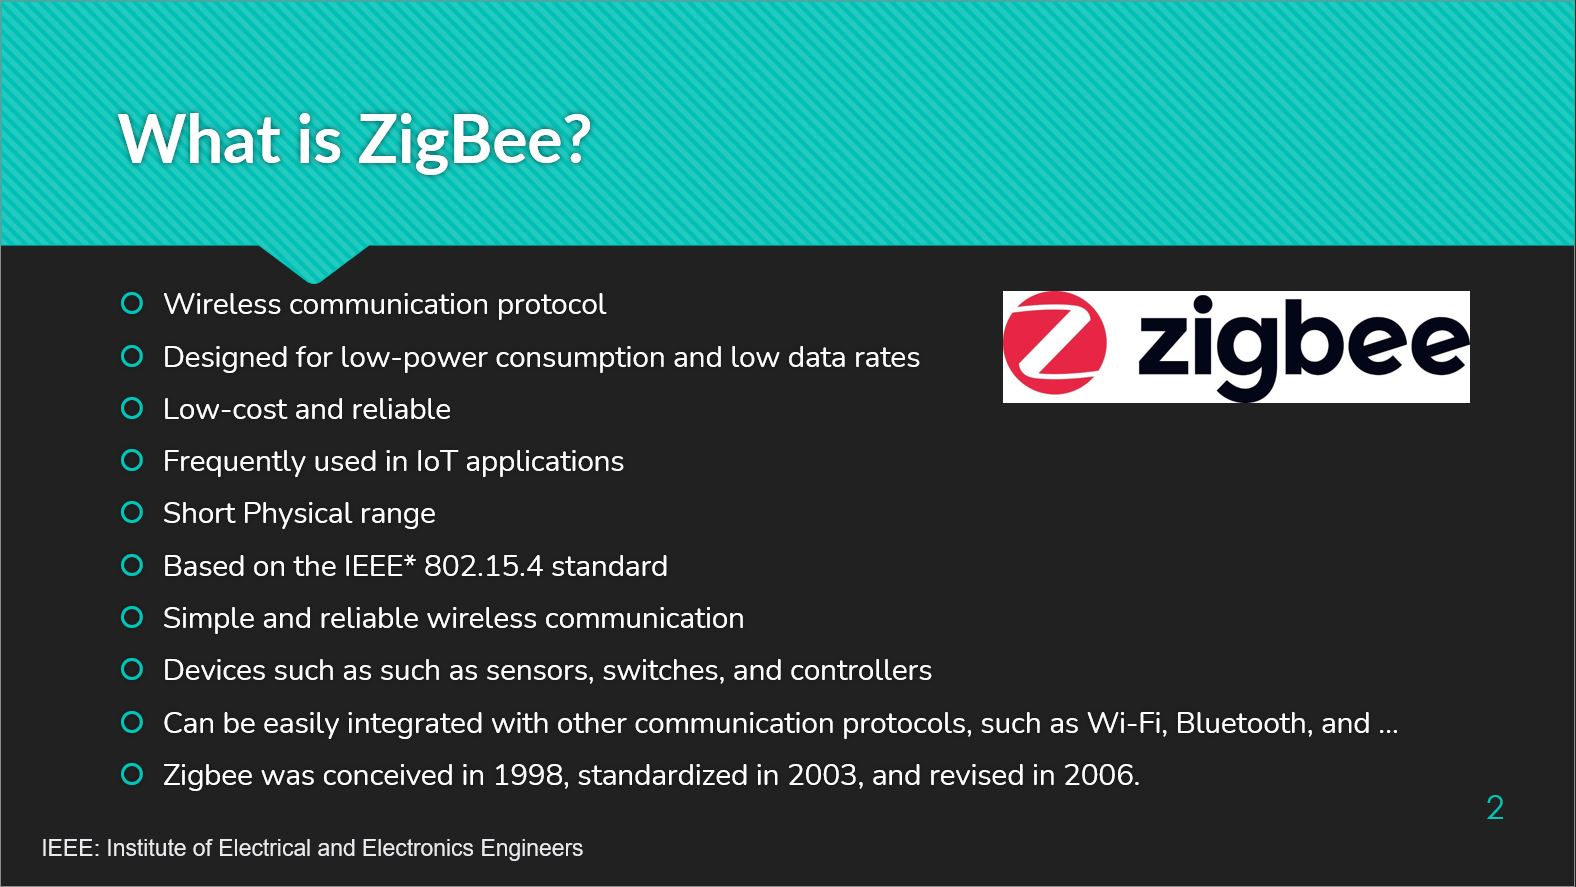
\includegraphics[width=1\linewidth]{images/sample.jpg}
    \caption{یک نمونه از اسلاید های ارائه }
    \label{fig:h}
\end{figure}


